%%%%%%%%%%%%%%%%%%%%%%%%%%%%%%%%%%%%%%%%%%%%%%%%%%%%%%%%%%%
% --------------------------------------------------------
% Tau
% LaTeX Template
% Version 2.4.1 (22/05/2024)
%
% Author: 
% Guillermo Jimenez (memo.notess1@gmail.com)
% 
% License:
% Creative Commons CC BY 4.0
% --------------------------------------------------------
%%%%%%%%%%%%%%%%%%%%%%%%%%%%%%%%%%%%%%%%%%%%%%%%%%%%%%%%%%%
\documentclass[9pt,a4paper,twoside]{tau-class/tau}

%----------------------------------------------------------
% TITLE
%----------------------------------------------------------

\usepackage{enumitem}
\newcount\NewCount

\journalname{ESCOM}
\title{Problema de la Coloración Mínima}%! Modificar con el título del proyecto


%----------------------------------------------------------
% AUTHORS, AFFILIATIONS AND PROFESSOR
%----------------------------------------------------------

\author[a]{Diego Castillo Reyes}
\author[a]{Marthon Leobardo Yañez Martinez}
\author[a]{Aldo Escamilla Resendiz}
\author[a]{Muñoz González Eduardo}

%----------------------------------------------------------

\affil[a]{Investigadores en formación, ESCOM, IPN}


\professor{Dra. Miriam Pescador Rojas}

%----------------------------------------------------------
% FOOTER INFORMATION
%----------------------------------------------------------

\institution{Escuela Superior de Cómputo, IPN}
\footinfo{Problema de la Coloración Mínima}%! Modificar con el título del proyecto
\theday{Junio 25, 2024}
\course{Algoritmos Genéticos}

%----------------------------------------------------------
% ABSTRACT AND KEYWORDS
%----------------------------------------------------------

\begin{abstract}    
    En este trabajo se presenta el problema de la coloración mínima, el cual es un problema NP-completo. 
    Se propone una solución basada en algoritmos genéticos para encontrar la coloración mínima de un grafo.


\end{abstract}

%----------------------------------------------------------

\keywords{Coloración Mínima, Genéticos, Algoritmos, Grafos}%! Modificar con las palabras clave

%----------------------------------------------------------

\begin{document}	
    \maketitle 
    \thispagestyle{firststyle} 
    \tauabstract
%----------------------------------------------------------

\section{Introducción}

    El problema de la coloración mínima es un problema NP-completo, el cual consiste en asignar un color a cada vértice de un grafo de tal manera que dos vértices adyacentes no tengan el mismo color.
    El objetivo es encontrar la coloración mínima, es decir, la menor cantidad de colores posibles para colorear el grafo.
    Este problema es de gran importancia en la teoría de grafos, ya que tiene aplicaciones en la asignación de horarios, asignación de frecuencias, asignación de canales, entre otros.
    En este trabajo se propone una solución basada en PSO, un algoritmo de optimización basado en la inteligencia de enjambre, para encontrar la coloración mínima de un grafo.

\section{Antecedentes}

    En una pequeña ciudad de Rusia, K\"onigsberg (Actualmente Kaliningrado, Rusia), existen siete puentes que conectan cuatro islas. Un matemático llamado Leonhard Euler (1707-1783) 
    se preguntó si era posible recorrer todos los puentes una sola vez y regresar al punto de partida. 
    Euler demostró en 1736 que no era posible en su publicación \textit{Solutio problematis ad geometriam situs pertinentis} \cite{euler1736}, y 
    para ello utilizó un grafo para representar las islas y los puentes como se ve en la Figura~\ref*{fig:konigsberg}. 
    \begin{figure}[H]
        \centering
        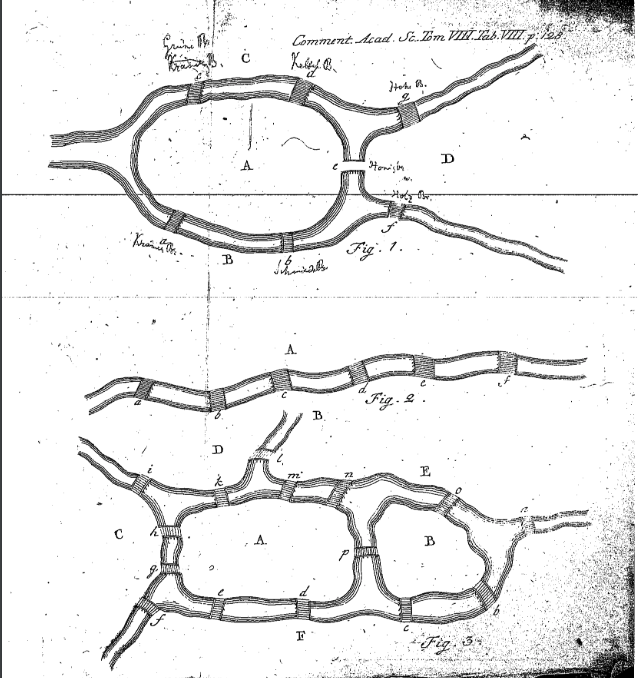
\includegraphics[width=0.5\columnwidth]{Images/Proy/Euler.png }
        \caption{Grafo de K\"onigsberg}
        \label{fig:konigsberg}
    \end{figure}
    Él demostró utilizando cada puente como una arista y cada isla como un vértice, que no era posible recorrer todos los puentes una sola vez y regresar al punto de partida.
    Siendo este el primer problema de teoría de grafos, el cual es un área de las matemáticas que estudia las relaciones entre los vértices y las aristas de un grafo.  
    Un grafo es un conjunto de vértices y aristas, donde las aristas son pares no ordenados de vértices.
    Posteriormente, en 1852, Francis Guthrie planteó el problema de los cuatro colores, el cual consiste en colorear un mapa de tal manera que dos regiones adyacentes no tengan el mismo color.
    Este problema fue resuelto en 1976 por Kenneth Appel y Wolfgang Haken utilizando una computadora, demostrando que cuatro colores son suficientes para colorear cualquier mapa~\cite{appel1976}.
    A partir de este problema, se han planteado diversos problemas de coloración, entre ellos el problema de la coloración mínima, el cual es un problema NP-completo.
    
\section{Metodología}

    Para poder resolver el problema de la coloración mínima, se propone una solución basada en algoritmos genéticos.
    El algoritmo genético elegido fue el de PSO (Particle Swarm Optimization), el cual es un algoritmo de optimización basado en la inteligencia de enjambre.
    El algoritmo PSO se basa en el comportamiento social de las partículas, las cuales se mueven en un espacio de búsqueda en busca de la mejor solución.
    Las partículas tienen mejoras cognitivas y mejoras sociales, las cuales les permiten moverse en el espacio de búsqueda.
    En el caso del problema de la coloración mínima, las partículas representan una coloración de un grafo, y el objetivo es encontrar la coloración mínima.
    La representación de las partículas es un vector de enteros que representa los colores de los vértices del grafo.
    El algoritmo PSO se encarga de mover las partículas en el espacio de búsqueda, de tal manera que se encuentre la coloración mínima del grafo.
    Para evaluar la calidad de una coloración, se utiliza la función objetivo, la cual es el número de colores utilizados en la coloración.

\section{Propuesta de solución}
% Usando listings agrega el código Proyecto\MCGP\mcgp.py
    \lstinputlisting[language=Python, caption=Algoritmo PSO para el problema de la coloración mínima, label=lst:pso]{MCGP/mcgp.py}



\section{Resultados}
% Agrega imagen graph.png
    \begin{figure}[H]
        \centering
        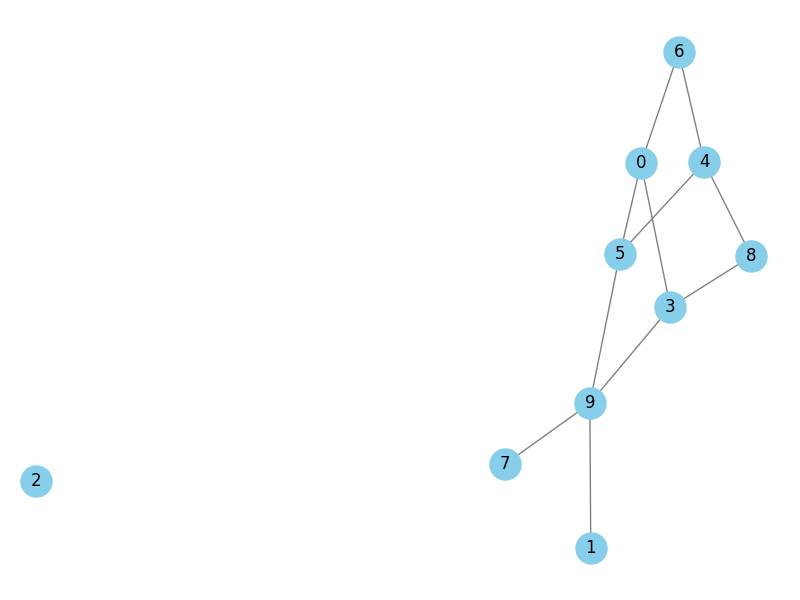
\includegraphics[width=0.5\columnwidth]{MCGP/graph.png}
        \caption{Grafo de 10 nodos}
        \label{fig:graph}
    \end{figure}
    En la Figura~\ref*{fig:graph} se muestra un grafo de 10 nodos que no es totalmente conexo, el cual 
    se utilizó para evaluar el algoritmo PSO propuesto.
% Agrega imagen graphColored.png
    \begin{figure}[H]
        \centering
        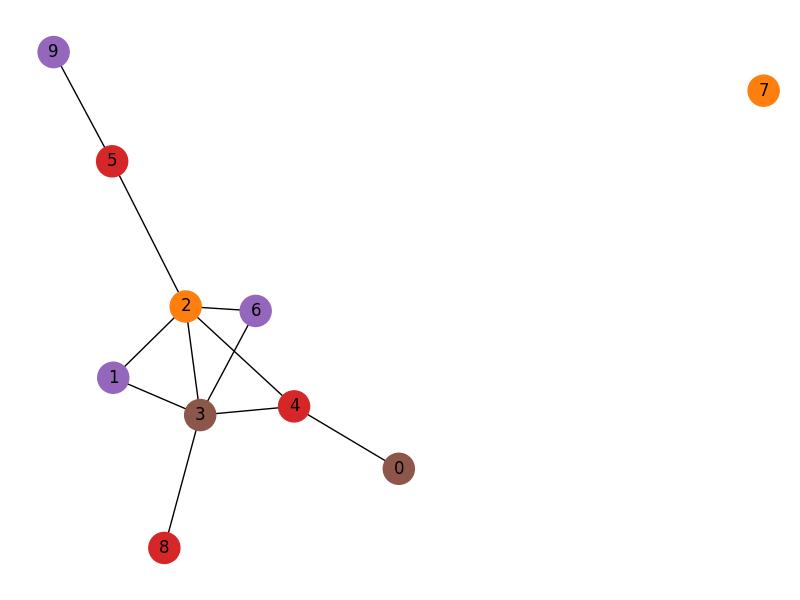
\includegraphics[width=0.5\columnwidth]{MCGP/graphColored.png}
        \caption{Coloración del grafo de 10 nodos}
        \label{fig:graphColored}
    \end{figure}
    En la Figura~\ref*{fig:graphColored} se muestra el resultado de la coloración del grafo de 10 nodos utilizando el algoritmo PSO propuesto.
    Como se puede observar, se utilizan 4 colores para colorear el grafo. \\ 
    En la salida de la terminal obtuvimos lo siguiente:
    % Usando listings agrega el txt MCGP/salida.txt
    \lstinputlisting[language=Python, caption=Salida del algoritmo PSO, label=lst:salida]{MCGP/salida.txt}

\section{Conclusiones}
    En conclusión, la coloración minima de grafos es un problema fundamental en la teoría de grafos y gracias a sus amplias aplicaciones como
    la asignación de horarios, asignación de frecuencias, asignación de canales, entre otros. Mediante la solución usando PSO hemos logrado solucionar el problema pasando de un tiempo NP 
    a un tiempo polinomial. 

\printbibliography

\end{document}